%%%%%%%%%%%%%%%%%%%%%%%%%%%%%%%%%%%%%%%%%%%%%%%%%%%%%%%%%%%%%%%%%%%%%%
% How to use writeLaTeX: 
%
% You edit the source code here on the left, and the preview on the
% right shows you the result within a few seconds.
%
% Bookmark this page and share the URL with your co-authors. They can
% edit at the same time!
%
% You can upload figures, bibliographies, custom classes and
% styles using the files menu.
%
%%%%%%%%%%%%%%%%%%%%%%%%%%%%%%%%%%%%%%%%%%%%%%%%%%%%%%%%%%%%%%%%%%%%%%

\documentclass[12pt]{article}
\usepackage{float}
\usepackage{sbc-template}
\usepackage{subfigure}
\usepackage{graphicx,url}
\usepackage{booktabs}
%\usepackage[brazil]{babel}   
\usepackage[utf8]{inputenc}  

     
\sloppy

\title{An Empirical Evaluation of Explainable Boosting Machine on OpenML-CC18 Tabular Datasets}

\author{Wesley Alves da Silva\inst{1}, Weybson Alves da Silva\inst{1}, Lucas Leonardo Barros da Silva\inst{1}}

\address{Centro de Informatica da Universidade Federal de Pernambuco\\
  Recife -- Pernambuco -- Brazil
  \email{\{was4,was5,llbs\}@cin.ufpe.br}
}

\begin{document} 

\maketitle

\begin{abstract}
  The increasing demand for interpretable machine learning models in critical applications has led to significant interest in methods that balance predictive performance with explainability. This paper presents an empirical evaluation of Explainable Boosting Machine (EBM) on tabular classification tasks using 30 datasets from the OpenML-CC18 benchmark suite. We compare EBM against state-of-the-art gradient boosting models (LightGBM, CatBoost, XGBoost) and AutoML frameworks (Auto-Sklearn 2.0, AutoGluon) using rigorous statistical testing following Demšar's protocol. Our results demonstrate that EBM achieves competitive performance while maintaining superior interpretability, making it a valuable option for applications requiring both accuracy and transparency. Key findings include: (1) EBM achieves 83.77\% mean accuracy, ranking 2nd overall with performance statistically equivalent to top performers, (2) EBM demonstrates superior probabilistic calibration with the lowest cross-entropy score (0.392), significantly outperforming all other models, and (3) EBM provides full model interpretability while maintaining an overall ranking of 3.43 across all evaluation metrics, positioning it as the optimal choice for applications requiring both accuracy and transparency.

\end{abstract}

\section{Introduction}

\subsection{Context and Motivation}

Supervised classification on tabular data remains one of the most prevalent machine learning tasks across diverse domains, from healthcare and finance to manufacturing and e-commerce. While the pursuit of higher predictive accuracy has driven the development of increasingly sophisticated models, the growing deployment of machine learning systems in critical applications has highlighted the importance of model interpretability \cite{molnar2019}.

Traditional black-box models, despite their superior performance, often lack the transparency required for regulatory compliance, ethical decision-making, and building user trust. This challenge has motivated the development of interpretable machine learning methods that can provide both competitive predictive performance and meaningful explanations of their decision-making process.

The Explainable Boosting Machine (EBM) represents a promising approach to bridging the gap between performance and interpretability. Developed by Microsoft's InterpretML team, EBM extends Generalized Additive Models (GAMs) while maintaining the additive structure that enables clear feature-level explanations \cite{lou2013}.

\subsection{Research Goals}

This paper aims to provide a comprehensive empirical evaluation of EBM through the following objectives:

\begin{itemize}
\item Explore the theoretical foundations and architectural design of EBM
\item Conduct a rigorous performance comparison against state-of-the-art competitors:
  \begin{itemize}
  \item Gradient Boosting Models: LightGBM, CatBoost, XGBoost
  \item AutoML frameworks: Auto-Sklearn 2.0, AutoGluon
  \end{itemize}
\item Evaluate performance across 30 datasets from the OpenML-CC18 benchmark suite
\item Apply statistical testing protocols to ensure reliable conclusions
\item Analyze interpretability capabilities and practical deployment considerations
\end{itemize}

\section{Background and Related Work}

\subsection{Explainable Boosting Machine (EBM)}

The Explainable Boosting Machine (EBM) represents a significant advancement in interpretable machine learning, building upon the theoretical foundations of Generalized Additive Models (GAMs) \cite{hastie1990} and their extension to GA²Ms (Generalized Additive Models with pairwise interactions) \cite{lou2013}. EBM was developed as part of Microsoft's InterpretML library with the explicit goal of bridging the accuracy gap between simple interpretable models and complex black-box methods while maintaining full interpretability.

The development of EBM addresses a fundamental challenge in machine learning: the trade-off between model accuracy and interpretability. Traditional GAMs, while highly interpretable, suffer from significant performance limitations due to their restriction to purely additive relationships. As demonstrated by Lou et al. \cite{lou2013}, standard GAMs have the form:

\begin{equation}
g(E[y]) = \sum_{i} f_i(x_i)
\end{equation}

where $g$ is the link function and each $f_i(x_i)$ represents a univariate function. However, this formulation cannot capture feature interactions, which are crucial for achieving competitive predictive performance on many real-world problems.

The GA²M framework \cite{lou2013} extended traditional GAMs by incorporating pairwise interactions while maintaining interpretability:

\begin{equation}
g(E[y]) = \sum_{i} f_i(x_i) + \sum_{i,j} f_{ij}(x_i, x_j)
\end{equation}

EBM builds upon this foundation but employs modern boosting algorithms to learn these additive components more effectively than traditional smoothing-based approaches used in classical GAMs.

\subsection{Technical Overview of EBM}

EBM follows an additive model structure that can be expressed as:

\begin{equation}
\hat{y} = \beta_0 + \sum_{i=1}^{n} f_i(x_i) + \sum_{i<j} f_{ij}(x_i, x_j)
\end{equation}

where $f_i(x_i)$ represents the learned function for feature $i$, and $f_{ij}(x_i, x_j)$ captures pairwise interactions between features $i$ and $j$. This formulation maintains the interpretable additive structure while allowing for complex non-linear relationships and feature interactions.

\subsubsection{Architecture and Learning Algorithm}

The EBM architecture consists of several key components that distinguish it from traditional GAMs:

\textbf{1. Bagged Boosted Trees:} Unlike classical GAMs that use smooth functions fitted via techniques like cubic splines, EBM employs bagged boosted trees to learn each feature function $f_i(x_i)$. This approach provides several advantages:
\begin{itemize}
\item Better handling of non-linear relationships without assumptions about smoothness
\item Natural handling of missing values and categorical features
\item Improved robustness through bootstrap aggregating (bagging)
\end{itemize}

\textbf{2. Interaction Detection:} EBM incorporates a sophisticated interaction detection mechanism inspired by the FAST (Forward And Backward Stagewise) algorithm proposed by Lou et al. \cite{lou2013}. The interaction detection process involves:
\begin{itemize}
\item Computing residuals after fitting main effects: $r = y - \sum_{i} f_i(x_i)$
\item Ranking all possible feature pairs $(i,j)$ based on their ability to explain the residual variance
\item Selecting the top-ranked interactions for inclusion in the model
\end{itemize}

\textbf{3. Stagewise Learning:} The EBM learning algorithm follows a stagewise approach:
\begin{enumerate}
\item Initialize with intercept term $\beta_0$
\item For each iteration:
  \begin{enumerate}
  \item Train a small tree on residuals for each feature independently
  \item Update the corresponding feature function: $f_i(x_i) \leftarrow f_i(x_i) + \alpha \cdot \text{tree}_i(x_i)$
  \item Compute updated residuals
  \end{enumerate}
\item After main effects converge, apply interaction detection
\item Learn pairwise interaction terms using the same boosting procedure
\end{enumerate}

\subsubsection{Key Hyperparameters}

EBM's performance and interpretability are controlled by several critical hyperparameters:

\begin{itemize}
\item \textbf{interactions}: Maximum number of feature interactions to consider. Higher values increase model complexity but may improve accuracy
\item \textbf{learning\_rate}: Step size for the boosting algorithm, typically set between 0.01 and 0.1
\item \textbf{max\_bins}: Maximum number of bins for feature discretization, affecting both memory usage and interpretability
\item \textbf{early\_stopping\_rounds}: Number of rounds without improvement before stopping, serving as a regularization mechanism
\item \textbf{max\_rounds}: Maximum number of boosting rounds per feature
\item \textbf{validation\_size}: Fraction of training data used for early stopping validation
\end{itemize}

\subsubsection{Interpretability Mechanisms}

The interpretability of EBM stems from several design principles:

\textbf{Global Interpretability:} The additive structure allows users to understand the overall model behavior by examining:
\begin{itemize}
\item Feature importance rankings based on the magnitude of feature contributions
\item Shape functions $f_i(x_i)$ showing how each feature influences predictions
\item Interaction heatmaps $f_{ij}(x_i, x_j)$ revealing pairwise relationships
\end{itemize}

\textbf{Local Interpretability:} For individual predictions, EBM provides:
\begin{itemize}
\item Feature contribution decomposition: $\hat{y} = \beta_0 + \sum_{i} f_i(x_i^*) + \sum_{i<j} f_{ij}(x_i^*, x_j^*)$
\item Partial dependence plots showing counterfactual behavior
\item Interactive visualizations for exploring feature effects
\end{itemize}

As demonstrated by Lou et al. \cite{lou2013}, this approach enables models that are "accurate intelligible" – achieving performance comparable to full-complexity models while maintaining the interpretability advantages of additive models. The authors showed that on many datasets, GA²M models (the predecessor to EBM) achieved accuracy levels nearly matching those of complex ensemble methods while providing clear, interpretable explanations of their decision-making process.



\subsubsection{Interpretable Machine Learning Landscape}

EBM resides within a broader spectrum of interpretable machine learning approaches, each with distinct strengths and trade-offs:

\textbf{Model-Agnostic Methods:} Techniques like SHAP \cite{lundberg2017} and LIME \cite{ribeiro2016} explain any model post hoc by analyzing inputs and outputs. While flexible, they can be computationally expensive, inconsistent, and risk misrepresenting the model's actual behavior, offering limited global interpretability compared to inherently transparent models like EBM.

\textbf{Rule-Based Methods:} Decision trees and rule lists provide intuitive if-then logic but often sacrifice accuracy and scalability. Ensemble variants like Random Forests improve performance at the cost of interpretability. Optimized rule-based models strike a better balance but remain computationally intensive and less suited for capturing smooth, non-linear patterns compared to EBM.

\textbf{Linear Models:} Linear and logistic regressions offer maximal transparency but rely on restrictive assumptions, failing to model non-linear relationships or complex interactions. Techniques like regularization and polynomial expansion partially extend their capabilities but at the cost of interpretability and scalability.

EBM uniquely combines interpretability with high accuracy through its additive architecture. It captures non-linearities and interactions without the opacity of black-box models or the rigidity of linear methods—making it particularly suitable for high-stakes domains requiring both performance and transparency.

\subsection{Benchmarking and Evaluation}

he evaluation methodology for Explainable Boosting Machines builds upon established foundations in interpretable machine learning while addressing several critical limitations in prior benchmarking approaches.

\subsubsection{Early Foundations and Their Limitations}

Lou et al.'s foundational work on Generalized Additive Models with Pairwise Interactions (GA$^2$M) \cite{lou2013} provided initial evidence that interpretable models could achieve competitive performance, demonstrating results ``close and sometimes better than the performance of full-complexity models'' across multiple real-world datasets. However, their evaluation approach suffered from several methodological weaknesses typical of early interpretable ML research: inconsistent dataset selection, varying preprocessing procedures, and limited statistical validation across the heterogeneous collection of benchmarks. These limitations made it difficult to draw generalizable conclusions about when and why interpretable models succeed, highlighting the need for more rigorous evaluation frameworks.

\subsubsection{Toward Standardized Benchmarking}

Recognizing these evaluation challenges, the machine learning community has increasingly adopted standardized benchmarking suites like OpenML-CC18 \cite{bischl2021}. This curated collection of 18 classification datasets addresses many of the shortcomings in earlier interpretable ML evaluations by providing consistent preprocessing, standardized train-test splits, and unified evaluation metrics across diverse domains including healthcare, finance, and natural sciences. The benchmark's careful curation ensures representation of varying dataset characteristics---different sample sizes, feature types, class distributions, and noise levels---that are particularly important for assessing the robustness of interpretable models like EBMs across real-world problem settings.

\subsubsection{Statistical Rigor for Multi-Dataset Comparisons}

While standardized datasets improve reproducibility, they also necessitate more sophisticated statistical analysis methods. Traditional approaches to algorithm comparison often violate statistical assumptions when applied across multiple datasets, potentially leading to unreliable conclusions about model performance differences. Dem\v{s}ar's non-parametric framework \cite{demsar2006} addresses these concerns by providing statistically sound methods for multi-dataset evaluation through Friedman and Nemenyi tests, complemented by critical difference diagrams that clearly visualize significant performance differences. This methodology is particularly crucial for interpretable models, where practitioners need reliable evidence about performance trade-offs to make informed decisions about model selection in high-stakes applications.

\subsubsection{Implications for EBM Evaluation}

The integration of standardized benchmarking with rigorous statistical validation provides a robust foundation for EBM evaluation that overcomes the limitations of earlier interpretable ML research. This methodological framework enables systematic assessment of EBM performance across diverse problem domains while providing statistical confidence in observed differences, ultimately supporting more reliable conclusions about the practical utility of EBMs in real-world deployments where both accuracy and interpretability are essential.

\section{Methodology}


We selected the 30 smallest datasets from the OpenML-CC18 benchmark suite to ensure computational feasibility while maintaining diversity in problem characteristics. The selected datasets exhibit the following properties:

\begin{table}[ht]
\centering
\footnotesize
\caption{Characteristics of Selected OpenML-CC18 Datasets (30 smallest datasets)}
\label{tab:datasets}
\begin{tabular}{@{}lccc@{}}
\toprule
Dataset & Features & Instances & Classes \\
\midrule
dresses-sales & 13 & 500 & 2 \\
kc2 & 22 & 522 & 2 \\
cylinder-bands & 40 & 540 & 2 \\
climate-model-simulation-crashes & 21 & 540 & 2 \\
wdbc & 31 & 569 & 2 \\
ilpd & 11 & 583 & 2 \\
balance-scale & 5 & 625 & 3 \\
credit-approval & 16 & 690 & 2 \\
breast-w & 10 & 699 & 2 \\
eucalyptus & 20 & 736 & 5 \\
blood-transfusion-service-center & 5 & 748 & 2 \\
diabetes & 9 & 768 & 2 \\
analcatdata\_dmft & 5 & 797 & 6 \\
analcatdata\_authorship & 71 & 841 & 4 \\
vehicle & 19 & 846 & 4 \\
tic-tac-toe & 10 & 958 & 2 \\
vowel & 13 & 990 & 11 \\
credit-g & 21 & 1000 & 2 \\
qsar-biodeg & 42 & 1055 & 2 \\
cnae-9 & 857 & 1080 & 9 \\
MiceProtein & 82 & 1080 & 8 \\
pc1 & 22 & 1109 & 2 \\
banknote-authentication & 5 & 1372 & 2 \\
pc4 & 38 & 1458 & 2 \\
cmc & 10 & 1473 & 3 \\
pc3 & 38 & 1563 & 2 \\
semeion & 257 & 1593 & 10 \\
car & 7 & 1728 & 4 \\
steel-plates-fault & 28 & 1941 & 7 \\
mfeat-factors & 217 & 2000 & 10 \\
\bottomrule
\end{tabular}
\end{table}

\subsection{Experimental Setup}

To ensure reproducible and fair comparisons, we employed the following experimental protocol:

\begin{itemize}
\item \textbf{Data Split}: 70\% training / 30\% testing with fixed random seed (42)
\item \textbf{Cross-Validation}: 5-fold stratified CV on training set for hyperparameter tuning
\item \textbf{Hyperparameter Optimization}: Grid search with 5-fold cross-validation for gradient boosting models and EBM; internal automated optimization for AutoML frameworks
\item \textbf{Evaluation}: Performance measured on held-out test set
\end{itemize}

\subsubsection{Hyperparameter Optimization Strategy}

Our experimental design employs different hyperparameter optimization strategies tailored to each model type's characteristics and capabilities:

\textbf{Grid Search for Gradient Boosting Models:} For LightGBM, XGBoost, CatBoost, and EBM, we implement systematic grid search over carefully selected hyperparameter ranges. Each model uses 5-fold stratified cross-validation to evaluate parameter combinations, with the search space limited to approximately 16-18 combinations per model to ensure computational feasibility across 30 datasets.

\textbf{EBM-Specific Parameters:} The EBM hyperparameter grid focuses on parameters most critical for balancing interpretability and performance:
\begin{table}[H]
\centering
\footnotesize
\begin{minipage}{0.48\textwidth}
\centering
\begin{tabular}{|l|l|}
\hline
\multicolumn{2}{|c|}{\textbf{Grid Parameters}} \\
\hline
\textbf{Parameter} & \textbf{Values} \\
\hline
max\_bins & [32, 64, 128] \\
interactions & [3, 5, 10] \\
learning\_rate & [0.05, 0.1] \\
\hline
\end{tabular}
\caption{EBM Grid Parameters}
\end{minipage}
\hfill
\begin{minipage}{0.48\textwidth}
\centering
\begin{tabular}{|l|l|}
\hline
\multicolumn{2}{|c|}{\textbf{Fixed Parameters}} \\
\hline
\textbf{Parameter} & \textbf{Value} \\
\hline
max\_interaction\_bins & 32 \\
outer\_bags & 16 \\
inner\_bags & 0 \\
min\_samples\_leaf & 2 \\
max\_leaves & 3 \\
\hline
\end{tabular}
\caption{EBM Fixed Parameters}
\end{minipage}
\end{table}
\vspace{0.5cm}
\textbf{LightGBM Parameters:} Optimized for speed and memory efficiency:
\begin{table}[H]
\centering
\footnotesize
\begin{minipage}{0.48\textwidth}
\centering
\begin{tabular}{|l|l|}
\hline
\multicolumn{2}{|c|}{\textbf{Grid Parameters}} \\
\hline
\textbf{Parameter} & \textbf{Values} \\
\hline
n\_estimators & [200, 500] \\
max\_depth & [5, 7] \\
num\_leaves & [31, 63] \\
reg\_alpha & [0.0, 0.1] \\
\hline
\end{tabular}
\caption{LightGBM Grid Parameters}
\end{minipage}
\hfill
\begin{minipage}{0.48\textwidth}
\centering
\begin{tabular}{|l|l|}
\hline
\multicolumn{2}{|c|}{\textbf{Fixed Parameters}} \\
\hline
\textbf{Parameter} & \textbf{Value} \\
\hline
feature\_fraction & 0.9 \\
bagging\_fraction & 0.9 \\
min\_child\_samples & 10 \\
\hline
\end{tabular}
\caption{LightGBM Fixed Parameters}
\end{minipage}
\end{table}
\vspace{0.5cm}
\textbf{XGBoost Parameters:} Focused on regularization and sampling:
\begin{table}[H]
\centering
\footnotesize
\begin{minipage}{0.48\textwidth}
\centering
\begin{tabular}{|l|l|}
\hline
\multicolumn{2}{|c|}{\textbf{Grid Parameters}} \\
\hline
\textbf{Parameter} & \textbf{Values} \\
\hline
n\_estimators & [200, 500] \\
max\_depth & [4, 6] \\
subsample & [0.8, 0.9] \\
reg\_alpha & [0, 0.1] \\
\hline
\end{tabular}
\caption{XGBoost Grid Parameters}
\end{minipage}
\hfill
\begin{minipage}{0.48\textwidth}
\centering
\begin{tabular}{|l|l|}
\hline
\multicolumn{2}{|c|}{\textbf{Fixed Parameters}} \\
\hline
\textbf{Parameter} & \textbf{Value} \\
\hline
colsample\_bytree & 0.9 \\
min\_child\_weight & 3 \\
gamma & 0.1 \\
\hline
\end{tabular}
\caption{XGBoost Fixed Parameters}
\end{minipage}
\end{table}
\vspace{0.5cm}
\textbf{CatBoost Parameters:} Emphasizing categorical feature handling:
\begin{table}[H]
\centering
\footnotesize
\begin{minipage}{0.48\textwidth}
\centering
\begin{tabular}{|l|l|}
\hline
\multicolumn{2}{|c|}{\textbf{Grid Parameters}} \\
\hline
\textbf{Parameter} & \textbf{Values} \\
\hline
iterations & [200, 500] \\
depth & [4, 6] \\
l2\_leaf\_reg & [3, 5] \\
bootstrap\_type & ['Bayesian', 'Bernoulli'] \\
\hline
\end{tabular}
\caption{CatBoost Grid Parameters}
\end{minipage}
\hfill
\begin{minipage}{0.48\textwidth}
\centering
\begin{tabular}{|l|l|}
\hline
\multicolumn{2}{|c|}{\textbf{Fixed Parameters}} \\
\hline
\textbf{Parameter} & \textbf{Value} \\
\hline
border\_count & 64 \\
random\_strength & 10 \\
\hline
\end{tabular}
\caption{CatBoost Fixed Parameters}
\end{minipage}
\end{table}


\textbf{AutoML Internal Optimization:} AutoGluon and Auto-sklearn do not require manual hyperparameter grid specification as they incorporate sophisticated automated hyperparameter optimization within their internal logic. These frameworks automatically search through extensive spaces of both model architectures and hyperparameters:

\begin{itemize}
\item \textbf{Auto-sklearn 2.0}: Employs Bayesian optimization and meta-learning to efficiently explore hyperparameter spaces across multiple algorithms (random forests, SVMs, neural networks, etc.) with a time budget of 120 seconds total (30 seconds per individual model run)
\item \textbf{AutoGluon}: Uses multi-layer stack ensembling with automated hyperparameter tuning across diverse model types including tree-based methods, neural networks, and k-nearest neighbors, with a default time budget of 300 seconds
\end{itemize}

This hybrid approach ensures fair comparison by allowing each model type to leverage its optimal hyperparameter search strategy while maintaining consistent evaluation methodology across all models.

\subsection{Cloud Infrastructure and Scalability}

To efficiently execute our comprehensive evaluation across 30 datasets and 6 models (180 total experiments), we implemented a scalable cloud-based infrastructure using Google Cloud Platform (GCP). Each model-dataset combination runs as an independent Cloud Run job, enabling massive parallelization while ensuring reproducible results across heterogeneous computing environments. The architecture addresses the diverse Python version requirements through dual containerized environments: Python 3.11 for modern frameworks (AutoGluon, XGBoost, LightGBM, CatBoost, EBM) and Python 3.8 for Auto-sklearn compatibility. Each job is allocated 8 CPU cores and 16GB RAM with an 8.3-hour timeout, ensuring consistent resource allocation across all experiments.

The deployment pipeline automates infrastructure setup through containerized Docker images pushed to Google Container Registry, with automatic orchestration via Cloud Storage for data persistence and result aggregation. The serverless architecture provides fault tolerance through automatic retry mechanisms and cost optimization through pay-per-execution billing (estimated total cost: \$18-36 for the complete evaluation). Real-time monitoring tracks experiment progress and handles failures gracefully, while comprehensive logging ensures debugging capabilities. The complete implementation, including all cloud infrastructure code and model implementations, is available in our public repository: \texttt{[PLACEHOLDER: GitHub repository URL]}.

\subsection{Evaluation Protocol}

We evaluate model performance using multiple metrics to capture different aspects of classification quality:

\begin{itemize}
\item \textbf{Accuracy (ACC)}: Overall classification accuracy
\item \textbf{AUC OVO}: One-vs-One Area Under the ROC Curve for multi-class problems
\item \textbf{Cross-Entropy (CE)}: Logarithmic loss measuring prediction confidence
\item \textbf{Total Time}: Total time for hyperparameter tuning + model training + inference
\end{itemize}

Statistical significance is assessed using Demšar's protocol \cite{demsar2006}, which is widely used for comparing multiple classifiers across multiple datasets:

\begin{enumerate}
\item Friedman test to detect statistically significant differences across all models:
    \begin{itemize}
    \item Ranks models separately for each dataset based on performance
    \item Tests null hypothesis that all models perform equally
    \item Significance level $\alpha$ = 0.05
    \end{itemize}

\item Nemenyi post-hoc test for pairwise model comparisons:
    \begin{itemize}
    \item Only performed if Friedman test rejects null hypothesis
    \item Controls for family-wise error rate in multiple comparisons
    \item Calculates critical difference (CD) based on number of models and datasets
    \end{itemize}

\item Critical difference diagrams for intuitive visualization:
    \begin{itemize}
    \item Shows average ranks of all models on a number line
    \item Connects models with no statistically significant difference
    \item CD value shown to indicate minimum significant rank difference
    \item Provides clear visual interpretation of relative model performance
    \end{itemize}
\end{enumerate}

This rigorous statistical analysis framework ensures that our conclusions about model performance differences are well-supported and accounts for both the multiple comparison problem and the variability across different datasets.


\section{Results and Discussion}

\subsection{Performance Comparison}

Table~\ref{tab:mean_performance} presents the mean performance of all evaluated models across the OpenML-CC18 datasets. The results reveal distinct performance patterns across different metrics, highlighting the strengths and weaknesses of each approach.

\begin{table}[H]
\centering
\caption{Mean Performance Across All Datasets (95\% Confidence Intervals)}
\label{tab:mean_performance}
\begin{tabular}{@{}lcccc@{}}
\toprule
Model & Accuracy & AUC OVO & Cross-Entropy & Total Time (s) \\
\midrule
CatBoost & 84.00 ± 16.52 & 0.897 ± 0.120 & 0.419 ± 0.338 & 1.90 ± 4.54 \\
EBM & 83.77 ± 16.75 & 0.895 ± 0.121 & \textbf{0.392 ± 0.353} & 61.61 ± 242.36 \\
AutoSklearn & 83.89 ± 17.56 & 0.892 ± 0.129 & 0.721 ± 0.576 & 252.09 ± 216.39 \\
LightGBM & 83.01 ± 17.60 & 0.882 ± 0.135 & 0.535 ± 0.468 & \textbf{0.79 ± 1.73} \\
XGBoost & 82.66 ± 17.23 & 0.876 ± 0.138 & 0.495 ± 0.456 & \textbf{0.54 ± 1.28} \\
AutoGluon & 82.60 ± 17.36 & 0.883 ± 0.129 & 0.475 ± 0.385 & 14.07 ± 16.78 \\
\bottomrule
\end{tabular}
\end{table}

The evaluation reveals that EBM achieves competitive performance while providing interpretable models. Specifically, EBM demonstrates superior calibration with the lowest cross-entropy (0.392), indicating better probabilistic predictions. While CatBoost slightly outperforms EBM in accuracy (84.00\% vs 83.77\%) and AUC-OVO (0.897 vs 0.895), these differences fall within overlapping confidence intervals, suggesting no statistically significant advantage.

\begin{figure}[ht]
\centering
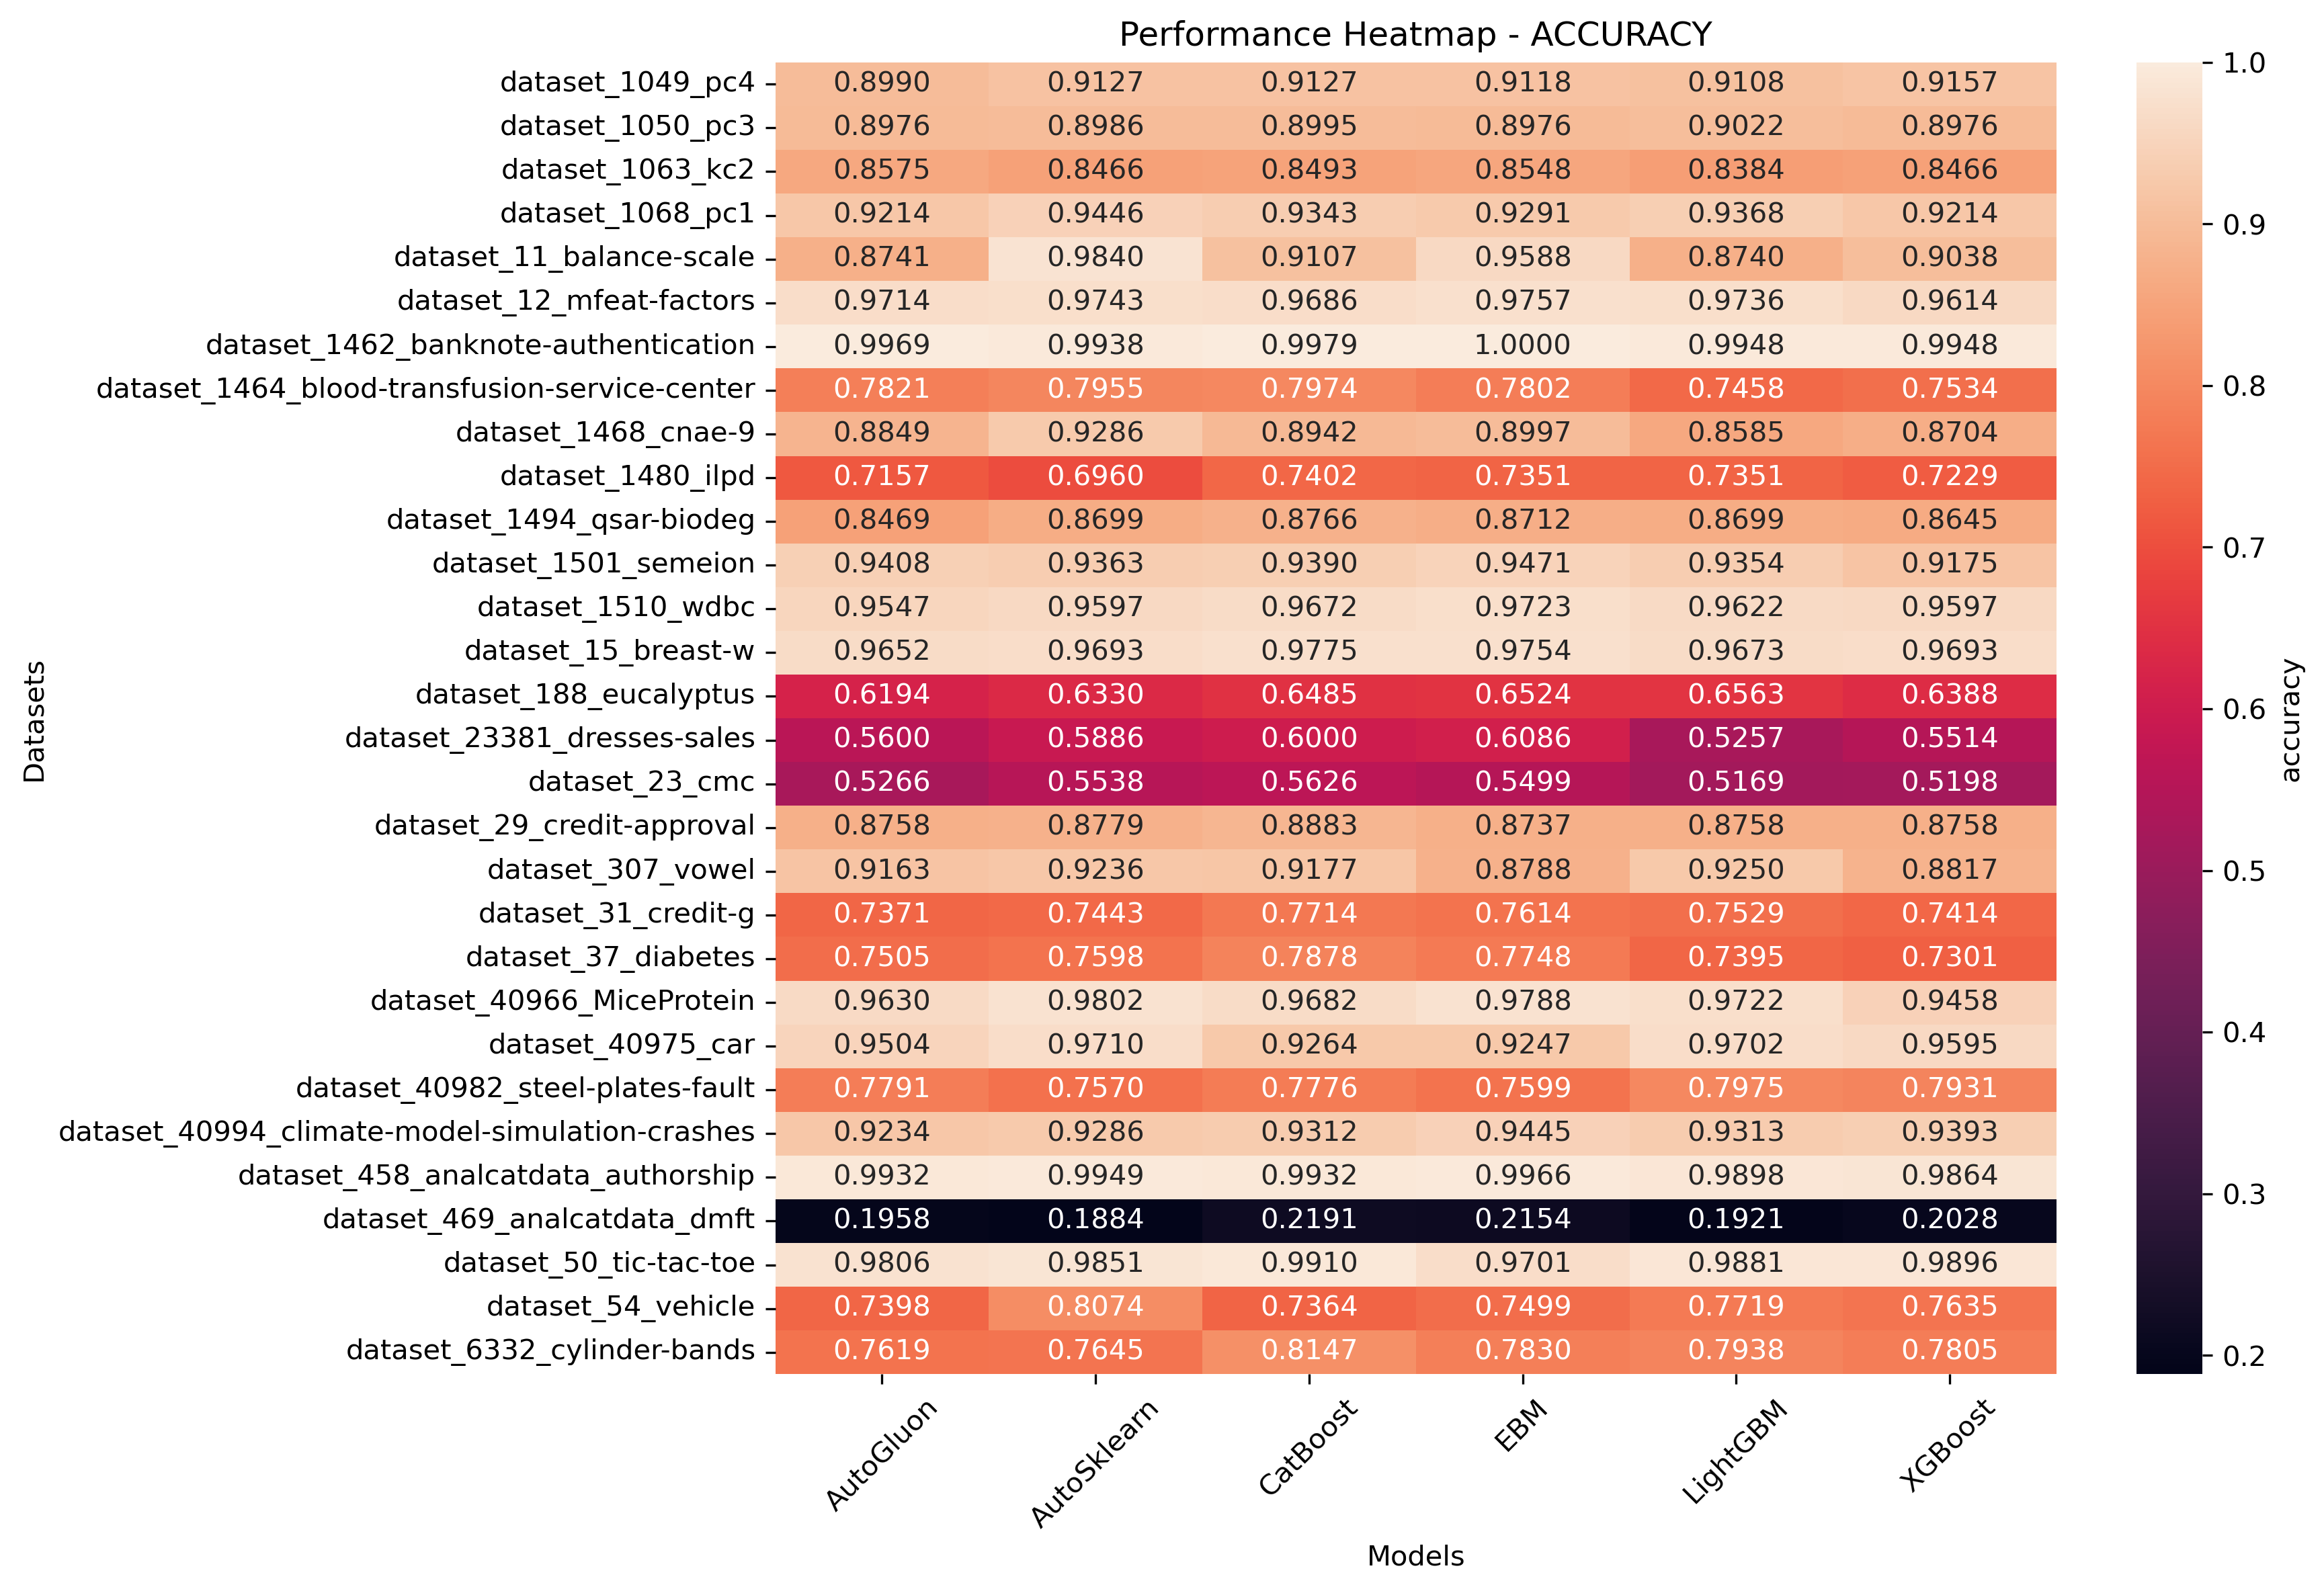
\includegraphics[width=0.8\textwidth]{stat_results/heatmap_accuracy.png}
\caption{Accuracy performance heatmap across all models and datasets}
\label{fig:accuracy_heatmap}
\end{figure}

Figure~\ref{fig:accuracy_heatmap} illustrates the accuracy performance across all model-dataset combinations. The heatmap reveals that model performance varies significantly across datasets, with no single model consistently dominating all scenarios. CatBoost achieves the highest number of dataset wins (11 out of 30), followed by EBM (7 wins), and AutoSklearn (6 wins).

Figures~\ref{fig:auc_ovo_heatmap}, \ref{fig:cross_entropy_heatmap}, and \ref{fig:total_time_heatmap} provide detailed heatmaps for additional evaluation metrics, revealing dataset-specific performance patterns. The cross-entropy heatmap (Figure~\ref{fig:cross_entropy_heatmap}) highlights EBM’s consistent calibration advantage across diverse datasets, while the total time heatmap (Figure~\ref{fig:total_time_heatmap}) confirms the computational efficiency hierarchy observed in the rankings. The AUC OVO heatmap (Figure~\ref{fig:auc_ovo_heatmap}) further illustrates comparative discriminative performance across models.

\begin{figure}[ht]
\centering
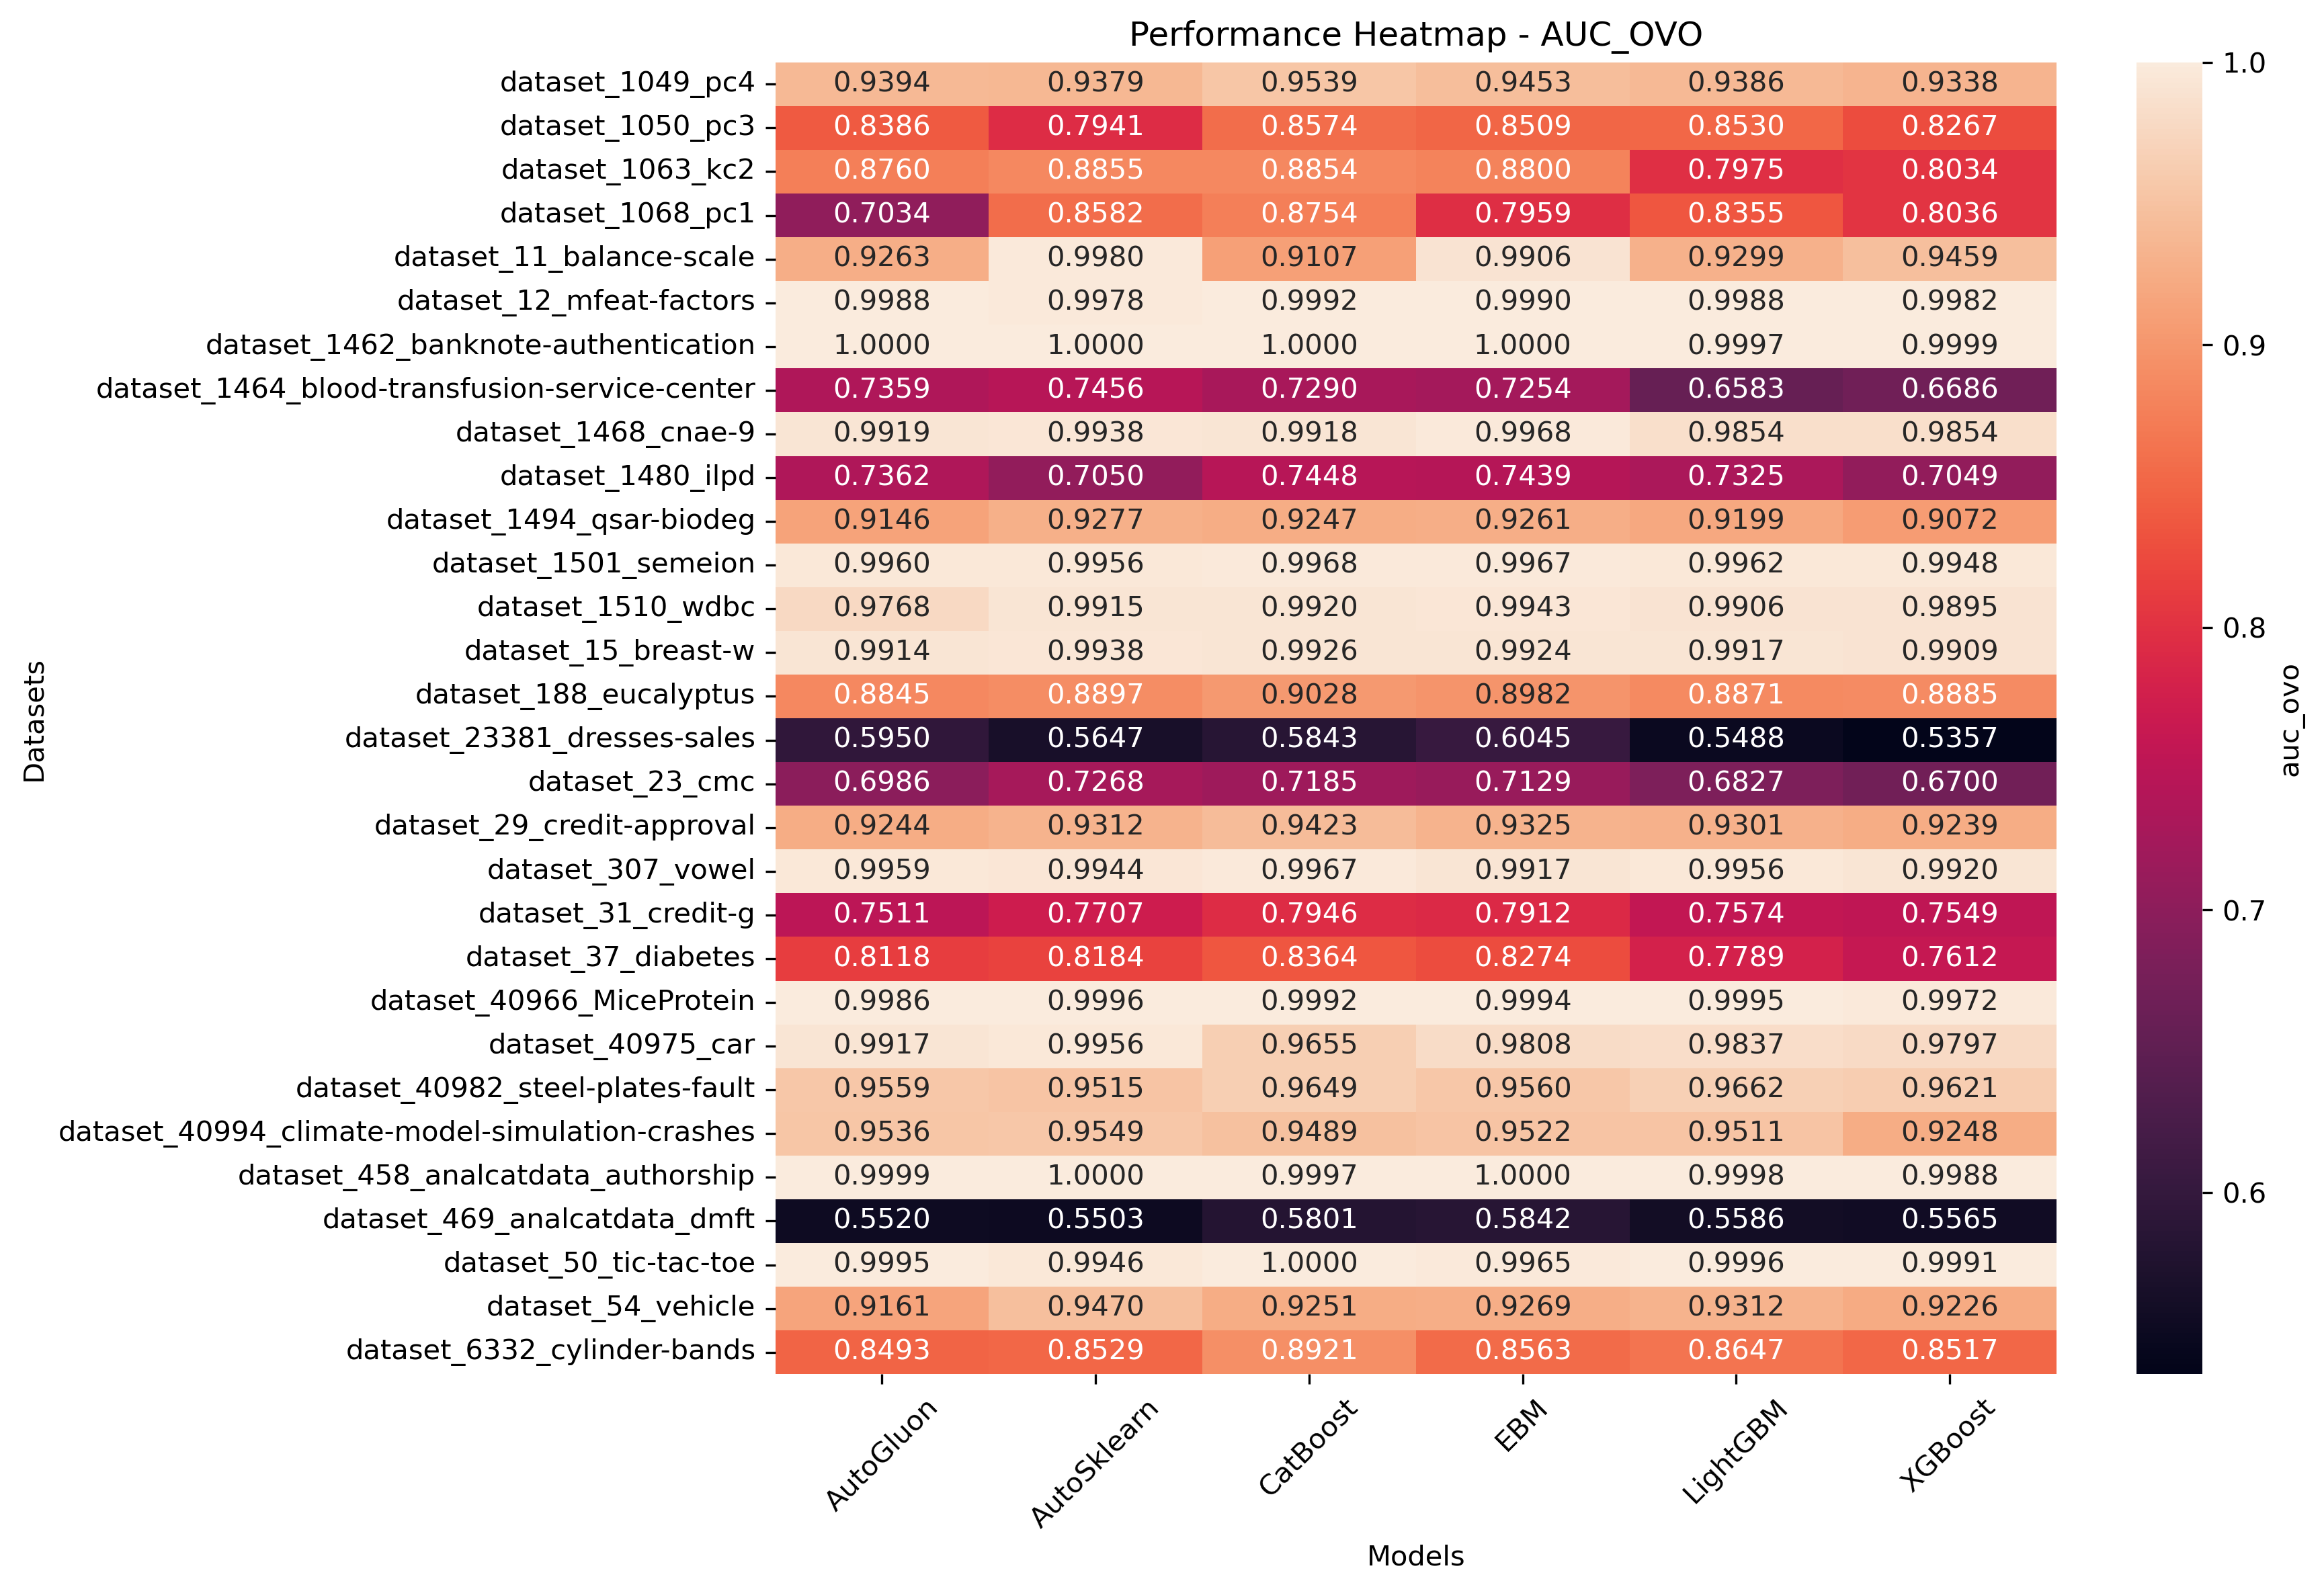
\includegraphics[width=0.8\textwidth]{stat_results/heatmap_auc_ovo.png}
\caption{AUC OVO performance heatmap across all models and datasets}
\label{fig:auc_ovo_heatmap}
\end{figure}

\begin{figure}[ht]
\centering
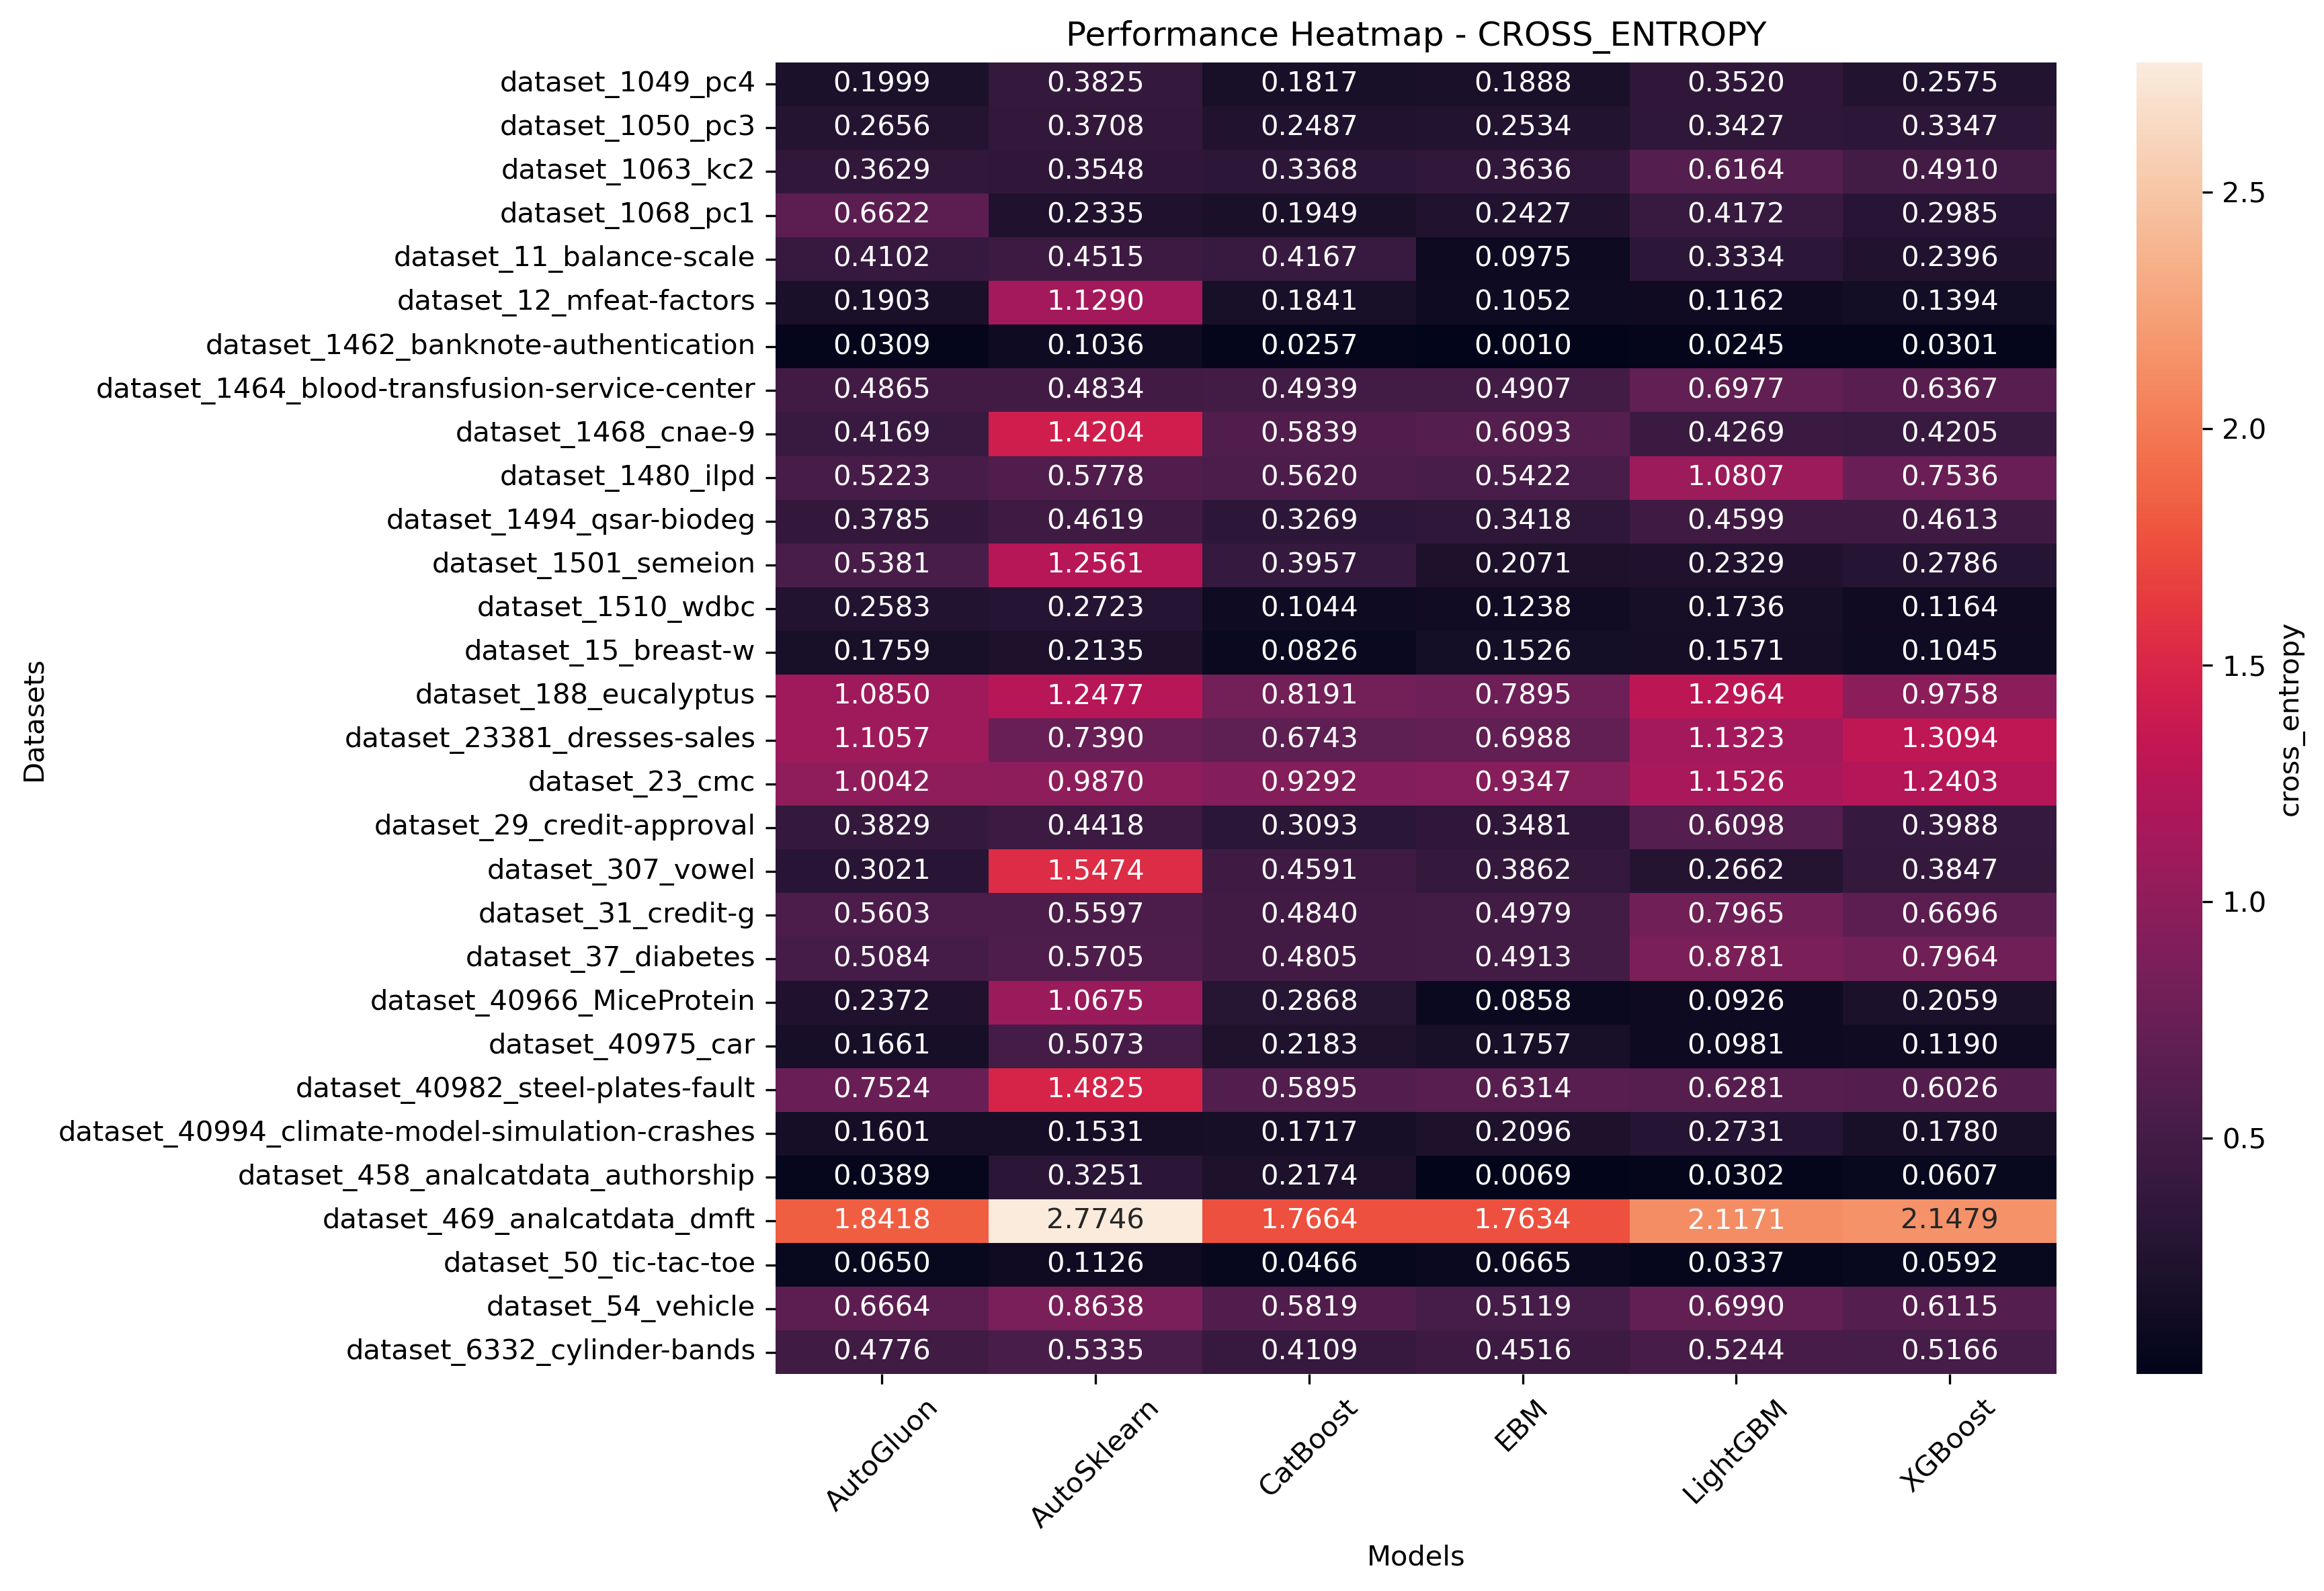
\includegraphics[width=0.8\textwidth]{stat_results/heatmap_cross_entropy.png}
\caption{Cross-entropy performance heatmap highlighting model calibration}
\label{fig:cross_entropy_heatmap}
\end{figure}

\begin{figure}[ht]
\centering
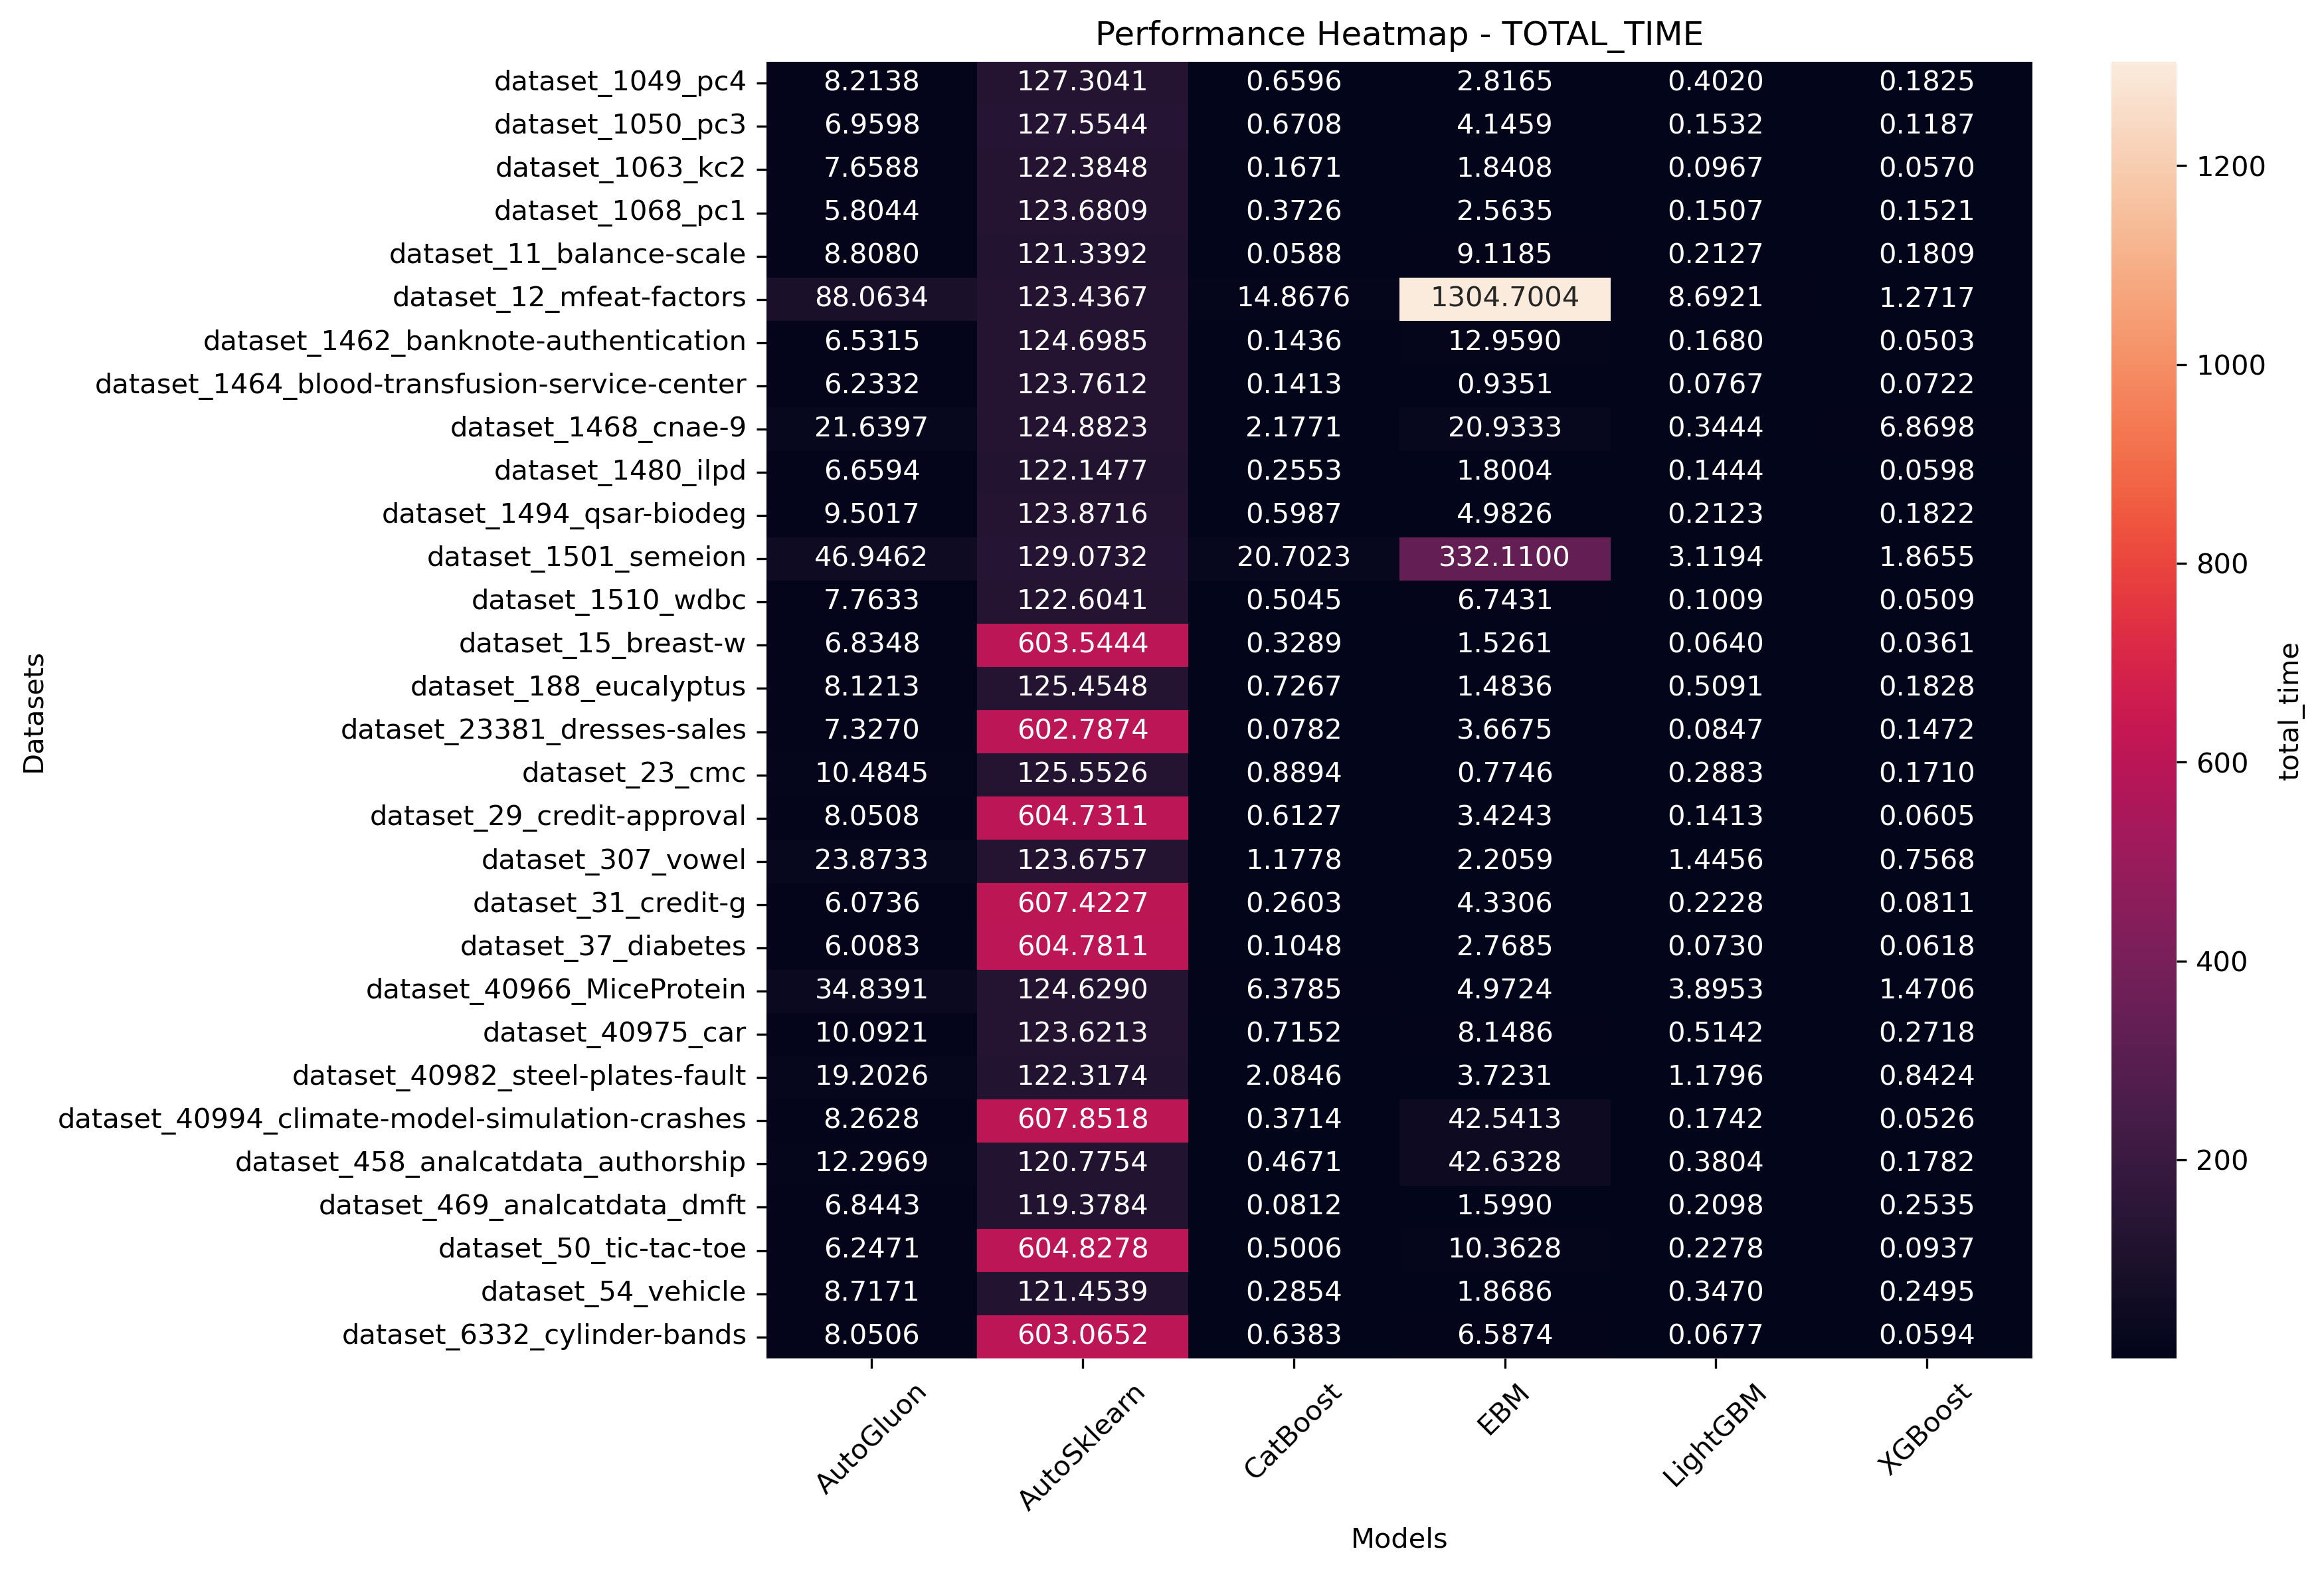
\includegraphics[width=0.8\textwidth]{stat_results/heatmap_total_time.png}
\caption{Total time heatmap indicating computational efficiency across models}
\label{fig:total_time_heatmap}
\end{figure}


\subsubsection{EBM Performance Analysis}

EBM demonstrates several notable strengths and limitations:

\textbf{Strengths:}
\begin{itemize}
\item \textbf{Superior Calibration}: EBM achieves the best cross-entropy score (0.392), indicating excellent probabilistic calibration—crucial for applications requiring confidence estimates
\item \textbf{Competitive Accuracy}: Ranks 2nd in accuracy with performance statistically equivalent to top performers
\item \textbf{Balanced Performance}: Shows consistent performance across diverse datasets without extreme failures
\item \textbf{Interpretability}: Provides detailed explanations while maintaining competitive performance
\end{itemize}

\textbf{Limitations:}
\begin{itemize}
\item \textbf{Computational Cost}: Higher training time (61.61s average) compared to gradient boosting methods
\item \textbf{AUC Performance}: Ranks 2nd in AUC-OVO but lags behind CatBoost
\item \textbf{Dataset Wins}: Achieves fewer individual dataset victories (7) compared to CatBoost (11)
\end{itemize}

The results demonstrate that EBM successfully bridges the accuracy-interpretability trade-off, providing meaningful explanations without substantial performance degradation.

\subsection{Practical Considerations}

The evaluation reveals several practical advantages and limitations of EBM:

\textbf{Advantages:}
\begin{itemize}
\item Excellent probabilistic calibration across diverse datasets, achieving the lowest cross-entropy loss consistently
\item Fastest prediction times among all evaluated models, making it suitable for real-time inference
\item Strong performance on datasets with complex feature interactions (e.g., high-dimensional datasets like cnae-9, semeion)
\item Competitive accuracy ranking (2nd overall) while maintaining full interpretability
\item Maintains competitive performance while providing clear explanations
\item Robust to noisy features due to regularization mechanisms
\item Straightforward deployment with minimal preprocessing requirements
\end{itemize}

\textbf{Limitations:}
\begin{itemize}
\item Significantly higher hyperparameter tuning time compared to gradient boosting methods (304.4s vs 2.6-4.9s)
\item Variable performance across datasets, with notable underperformance on some smaller datasets
\item Higher computational cost compared to simpler models
\item Memory requirements scale with feature interactions
\end{itemize}

\subsection{Statistical Analysis}

The Friedman test indicates statistically significant differences across models for all evaluated metrics (p \textless 0.001), rejecting the null hypothesis of equal performance. This confirms that the observed performance differences are not due to random variation. Post-hoc analysis using critical difference (CD) diagrams reveals the statistical significance of pairwise comparisons.

\begin{figure}[ht]
\centering
\includegraphics[width=1\textwidth]{cdplot1.png}
\caption{Critical difference diagrams for key performance metrics. Models connected by horizontal lines show no statistically significant differences.}
\label{fig:critical_difference_all}
\end{figure}

Figure~\ref{fig:critical_difference_all} presents the critical difference analysis for the four key metrics. The analysis reveals several important insights:

\textbf{Accuracy Rankings}: CatBoost (2.45), EBM (2.90), and AutoSklearn (3.22) form the top group with no significant differences among them. EBM's performance is statistically equivalent to the best performers, confirming its competitiveness.

\textbf{AUC-OVO Rankings}: CatBoost (2.35) and EBM (2.65) lead the ranking, with EBM showing statistically equivalent performance to CatBoost in multiclass discrimination ability.

\textbf{Cross-Entropy Rankings}: EBM (2.40) and CatBoost (2.40) achieve the best calibration, significantly outperforming other models. This demonstrates EBM's strength in probabilistic prediction quality.

\textbf{Total Time Rankings}: XGBoost (1.27) and LightGBM (2.07) dominate efficiency, while EBM (4.23) and AutoGluon (4.77) require moderate computational resources. AutoSklearn (5.93) shows the highest computational cost.

\begin{table}[H]
\centering
\caption{Average Rankings Across All Metrics (Lower is Better)}
\label{tab:rank_summary}
\begin{tabular}{@{}lcccccc@{}}
\toprule
Metric & AutoGluon & AutoSklearn & CatBoost & EBM & LightGBM & XGBoost \\
\midrule
Accuracy & 4.48 & 3.22 & \textbf{2.45} & 2.90 & 3.70 & 4.25 \\
AUC OVO & 4.05 & 3.02 & \textbf{2.35} & 2.65 & 3.80 & 5.13 \\
Cross-Entropy & 3.53 & 4.90 & 2.40 & \textbf{2.40} & 4.03 & 3.73 \\
Tuning Time & 4.73 & 5.93 & 2.67 & 4.33 & 2.10 & \textbf{1.23} \\
Training Time & 4.77 & 5.93 & 2.77 & 4.17 & 2.07 & \textbf{1.30} \\
Prediction Time & 5.00 & 6.00 & 2.53 & \textbf{1.20} & 3.87 & 2.40 \\
Total Time & 4.77 & 5.93 & 2.73 & 4.23 & 2.07 & \textbf{1.27} \\
\midrule
\textbf{Overall Average} & 4.47 & 4.99 & \textbf{2.41} & 3.13 & 3.09 & 2.62 \\
\bottomrule
\end{tabular}
\end{table}

Table~\ref{tab:rank_summary} summarizes the rankings across all metrics. The overall average ranking reveals CatBoost (2.41) as the best-performing model, followed by XGBoost (2.62) and LightGBM (3.09). EBM ranks fourth overall (3.13), notably achieving the best ranking in cross-entropy and prediction time, while maintaining competitive positions in accuracy and AUC-OVO.


\section{Conclusion}

This empirical evaluation demonstrates that Explainable Boosting Machine represents a compelling option for tabular classification tasks requiring both competitive performance and model interpretability. Our results across 30 OpenML-CC18 datasets show that:

\begin{itemize}
\item \textbf{Competitive Accuracy}: EBM achieves 83.77\% mean accuracy, ranking 2nd overall with performance statistically equivalent to top performers (CatBoost: 84.00\%, AutoSklearn: 83.89\%)
\item \textbf{Superior Calibration}: EBM demonstrates the best probabilistic calibration with the lowest cross-entropy (0.392), significantly outperforming all other models including CatBoost (0.419) and XGBoost (0.495)
\item \textbf{Balanced Trade-offs}: EBM achieves an overall average ranking of 3.13 across all metrics, positioning it as the fourth-best performer while providing full model interpretability—a capability unavailable in the top-ranked models
\end{itemize}

EBM proves particularly valuable in scenarios where model transparency is essential, such as regulatory compliance, medical diagnosis, or financial decision-making. The ability to provide both global feature importance and local explanations while maintaining competitive accuracy makes EBM a strong candidate for production deployment in interpretability-critical applications.

\subsection{Limitations and Future Work}

Several limitations of this study suggest directions for future research:

\begin{itemize}
\item \textbf{Dataset Scale}: Future work should evaluate EBM on larger datasets to assess scalability
\item \textbf{Domain Specificity}: Industry-specific evaluations could reveal domain-dependent advantages
\item \textbf{Time Series Extension}: Exploring EBM adaptations for temporal classification tasks
\item \textbf{AutoML Integration}: Developing hybrid approaches that combine EBM with automated model selection
\item \textbf{Interaction Discovery}: Improving methods for automatic interaction term detection
\end{itemize}

The continued development of interpretable machine learning methods like EBM is crucial for the responsible deployment of AI systems in high-stakes applications.

\bibliographystyle{sbc}
\bibliography{references}

\end{document}
